\section{Gestion des utilisateurs}\label{gestion-des-utilisateurs}

Unix est pensé pour supporter plusieurs utilisateurs. On doit d'abord
s'authentifier

\subsection{Authentification}\label{authentification}

On se connecte via un mot de passe en local ou distant (\emph{ssh}). Il
existe aussi les authentifications par données biométriques,
cryptographie asymétrique (private key and public key).

Le premier processus au démarrage est le processus de \texttt{login} qui
va lui fork tous les autres sous-processus. On liste tous les users dans
\texttt{/etc/passwd}. On y stockait avant les mots de passe dedans mais
maintenant on les stocke dans des fichiers séparés (\emph{shadow
password}).

\subsubsection{\texorpdfstring{\texttt{/etc/passwd}}{/etc/passwd}}\label{etcpasswd}

\texttt{oracle:x:1021:1020:Oracle\ user:/data/network/oracle:/bin/bash}

\texttt{1:2:3:4:5:6:7}

\begin{enumerate}
\def\labelenumi{\arabic{enumi}.}
\tightlist
\item
  Nom d'utilisateur
\item
  Mot de passe (stocké dans \texttt{/etc/shadow})
\item
  Identifiant User (\textbf{UID})
\item
  Identifiant du groupe \emph{principal} de l'user (\textbf{GID})
\item
  Informations supplémentaires, nom complet de l'user
\item
  Répertoire \emph{home}
\item
  Shell à exécuter au moment du login de l'user
\end{enumerate}

\subsubsection{Types d'user}\label{types-duser}

\begin{longtable}[]{@{}
  >{\centering\arraybackslash}p{(\columnwidth - 2\tabcolsep) * \real{0.1081}}
  >{\centering\arraybackslash}p{(\columnwidth - 2\tabcolsep) * \real{0.8919}}@{}}
\toprule\noalign{}
\begin{minipage}[b]{\linewidth}\centering
type d'user
\end{minipage} & \begin{minipage}[b]{\linewidth}\centering
Description
\end{minipage} \\
\midrule\noalign{}
\endhead
\bottomrule\noalign{}
\endlastfoot
root & Aucune restriction et peut tout faire. Admin du système. \\
User normal & Droit limité mais peut obtenir des droits de root via
\texttt{sudo}. \\
User système & Ne correspond pas un réel user mais correspond à des
services du SE. (typiquement des daemons, \ldots) \\
\end{longtable}

\paragraph{\texorpdfstring{Obtenir leur
\textbf{UID}}{Obtenir leur UID}}\label{obtenir-leur-uid}

On utilise la fonction \texttt{getuid(2)} pour obtenir l'\textbf{UID} et
\texttt{geteuid(2)} pour obtenir l'\emph{effective \textbf{UID}} car il
se peut que les droits changent temporairement (\texttt{sudo}).

\paragraph{\texorpdfstring{Changer
l'\textbf{UID}}{Changer l'UID}}\label{changer-luid}

On peut faire cela via \texttt{setuid(2)} qui modifie l'UID de
l'utilisateur en cours d'exécution. Donc Root appelle \texttt{setuid}
avant \texttt{execve} pour se donner les droits d'administration.

\section{Systèmes de fichiers}\label{systuxe8mes-de-fichiers}

Il y a énormément de diversité en terme de support de stockage de
données. Il faut donc une interface \emph{commune}. En \textbf{UNIX},
les fichiers sont regroupés sous forme d'une arborescence unique.

\subsection{Hiérarchie et Montage}\label{hiuxe9rarchie-et-montage}

\begin{figure}
\centering
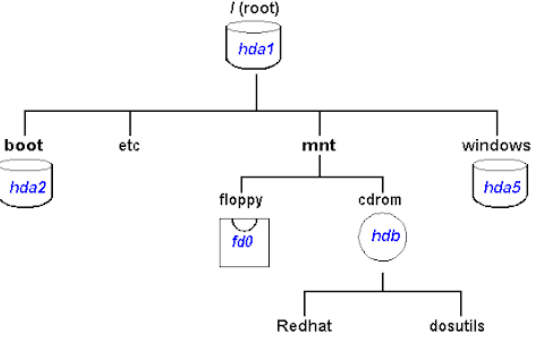
\includegraphics{image-34.png}
\caption{Alt text}
\end{figure}

En utilisant \texttt{mnt} on peut attacher ou détacher des systèmes de
fichiers dans la hiérarchie commune. Tout est un fichier en Linux (même
le \texttt{/proc}).

\subsection{contenu d'un répertoire}\label{contenu-dun-ruxe9pertoire}

\begin{verbatim}
$ ls -la / 
total 1488
drwxr-xr-x  19 root root    4096 Dec  9 14:35 .
drwxr-xr-x  19 root root    4096 Dec  9 14:35 ..
lrwxrwxrwx   1 root root       7 Apr 23  2020 bin -> usr/bin
drwxr-xr-x   2 root root    4096 Apr 23  2020 boot
drwxr-xr-x   9 root root    2820 Dec  9 14:35 dev
drwxr-xr-x 131 root root   12288 Dec  9 14:35 etc
drwxr-xr-x   3 root root    4096 Nov 15  2021 home
-rwxr-xr-x   3 root root 1440152 May  7  2022 init
lrwxrwxrwx   1 root root       7 Apr 23  2020 lib -> usr/lib
lrwxrwxrwx   1 root root       9 Apr 23  2020 lib32 -> usr/lib32
lrwxrwxrwx   1 root root       9 Apr 23  2020 lib64 -> usr/lib64
lrwxrwxrwx   1 root root      10 Apr 23  2020 libx32 -> usr/libx32
drwx------   2 root root   16384 Apr 10  2019 lost+found
drwxr-xr-x   2 root root    4096 Apr 23  2020 media
drwxr-xr-x   6 root root    4096 Sep 19 23:43 mnt
drwxr-xr-x   2 root root    4096 Apr 23  2020 opt
dr-xr-xr-x 244 root root       0 Dec  9 14:35 proc
drwx------   2 root root    4096 Feb 21  2023 root
drwxr-xr-x   6 root root     120 Dec  9 14:35 run
lrwxrwxrwx   1 root root       8 Apr 23  2020 sbin -> usr/sbin
drwxr-xr-x   2 root root    4096 Apr 10  2020 snap
drwxr-xr-x   2 root root    4096 Apr 23  2020 srv
dr-xr-xr-x  11 root root       0 Dec  9 14:35 sys
drwxrwxrwt  13 root root    4096 Dec  9 14:35 tmp
drwxr-xr-x  14 root root    4096 Apr 23  2020 usr
drwxr-xr-x  13 root root    4096 Apr 23  2020 var
\end{verbatim}

\subsubsection{Permissions}\label{permissions}

En analysant la première colonne, on peut savoir quelles sont les
permissions et si c'est un lien symbolique, hardlink ou directory.

On encode les permissions sur 9 bits via User (rwx), Groupe (rwx),
Autres (rwx). Ainsi, on connait les droits si on a le même UID, GUID ou
UID et GUID différents.

\begin{longtable}[]{@{}
  >{\centering\arraybackslash}p{(\columnwidth - 2\tabcolsep) * \real{0.0388}}
  >{\centering\arraybackslash}p{(\columnwidth - 2\tabcolsep) * \real{0.9612}}@{}}
\toprule\noalign{}
\begin{minipage}[b]{\linewidth}\centering
Droit
\end{minipage} & \begin{minipage}[b]{\linewidth}\centering
Description
\end{minipage} \\
\midrule\noalign{}
\endhead
\bottomrule\noalign{}
\endlastfoot
\texttt{r} & \emph{read}: lire le fichier, lister le contenu du
répertoire \\
\texttt{w} & \emph{write}: écrire dans le fichier, créer une entrée dans
le répertoire \\
\texttt{x} & \emph{execute}: accepter pour faire \texttt{execve} pour un
fichier. Pour un répertoire, on peut accéder à un fichier ou
sous-répertoire \\
\end{longtable}

\paragraph{\texorpdfstring{Subtilité du
\texttt{x}}{Subtilité du x}}\label{subtilituxe9-du-x}

\begin{verbatim}
$ mkdir -p repertoire 
$ echo "LINFO1252" > repertoire/fichier 
$ chmod 000 repertoire/ 
$ ls -al repertoire/
ls: cannot open directory repertoire/: Permission denied 
$ cat repertoire/fichier
cat: repertoire/fichier: Permission denied 
$ chmod +x repertoire/ 
$ ls -al repertoire/
ls: cannot open directory repertoire/: Permission denied
$ cat repertoire/fichier
LINFO1252
\end{verbatim}

\texttt{chmod} va changer les droits. On ne peut plus lister le fichier
car on a pas \texttt{r} mais on peut quand même y accéder car on a
\texttt{x} pour aller dans d'autres sous fichiers.

On représente les permissions comme 3 séquences de 3 bits donc
\texttt{rwxr-xr-\/-} = \texttt{754}. En utilisant \texttt{S\_ISUID} pour
un exécutable, permet l'exécution avec les permissions du propriétaire
de l'exécutable et pas celles de l'utilisateur.

\subsubsection{Navigation}\label{navigation}

Pour changer de répertoire en C où on exécute, on peut réaliser l'appel
suivant:

\begin{Shaded}
\begin{Highlighting}[]
\PreprocessorTok{\#include }\ImportTok{\textless{}unistd.h\textgreater{}}\PreprocessorTok{ }
\DataTypeTok{int}\NormalTok{ chdir}\OperatorTok{(}\DataTypeTok{const} \DataTypeTok{char} \OperatorTok{*}\NormalTok{path}\OperatorTok{);}
\end{Highlighting}
\end{Shaded}

\subsubsection{Fonctions Utiles}\label{fonctions-utiles}

\begin{longtable}[]{@{}
  >{\centering\arraybackslash}p{(\columnwidth - 2\tabcolsep) * \real{0.2966}}
  >{\centering\arraybackslash}p{(\columnwidth - 2\tabcolsep) * \real{0.7034}}@{}}
\toprule\noalign{}
\begin{minipage}[b]{\linewidth}\centering
Fonction
\end{minipage} & \begin{minipage}[b]{\linewidth}\centering
description
\end{minipage} \\
\midrule\noalign{}
\endhead
\bottomrule\noalign{}
\endlastfoot
\texttt{stat} & récupère les méta-données associées à un fichier ou
répertoire \\
\texttt{chmod}/\texttt{chown} & modifier les permissions ou le
propriétaire/groupe \\
\texttt{utime} & modifier les dates de création/modifications d'un
fichier (e.g.~commande \texttt{touch}) \\
\texttt{rename} & changer de nom, d'emplacement \\
\texttt{mkdir}/\texttt{rmdir} & créer/détruire un répertoire \\
\texttt{opendir}/\texttt{closedir}/\texttt{readir} & consulter le
contenu des répertoires \\
\end{longtable}

\subsubsection{Parcours de répertoire}\label{parcours-de-ruxe9pertoire}

\begin{Shaded}
\begin{Highlighting}[]
\KeywordTok{struct}\NormalTok{ dirent }\OperatorTok{\{} 
\NormalTok{    ino\_t d\_ino}\OperatorTok{;}                \CommentTok{/* inode number */}
\NormalTok{    off\_t d\_off}\OperatorTok{;}                \CommentTok{/* offset to the next dirent */} 
    \DataTypeTok{unsigned} \DataTypeTok{short}\NormalTok{ d\_reclen}\OperatorTok{;}    \CommentTok{/* length of this record */}
    \DataTypeTok{unsigned} \DataTypeTok{char}\NormalTok{ d\_type}\OperatorTok{;}       \CommentTok{/* type of file; not supported by all file system types */}
    \DataTypeTok{char}\NormalTok{ d\_name}\OperatorTok{[}\DecValTok{256}\OperatorTok{];}           \CommentTok{/* filename */}
\OperatorTok{\};}
\end{Highlighting}
\end{Shaded}

Il faut d'abord avoir ouvert un répertoire via \texttt{opendir}.
\texttt{readdir} pour accéder aux entrées du système.

La fonction \texttt{readdir} \textbf{n'est pas thread-safe}. On ne peut
donc pas appeler la fonction dans un autre thread quand cette dernière
est déjà en cours d'exécution quelque part (on utilise de la mémoire
statique). Il existe \texttt{readdir\_r} qui utilise un pointeur vers
une zone mémoire allouée qui est thread-safe.

\begin{Shaded}
\begin{Highlighting}[]
\DataTypeTok{int}\NormalTok{ readdir\_r}\OperatorTok{(}\NormalTok{DIR }\OperatorTok{*}\DataTypeTok{restrict}\NormalTok{ dirp}\OperatorTok{,} \KeywordTok{struct}\NormalTok{ dirent }\OperatorTok{*}\DataTypeTok{restrict}\NormalTok{ entry}\OperatorTok{,} \KeywordTok{struct}\NormalTok{ dirent }\OperatorTok{**}\DataTypeTok{restrict}\NormalTok{ result}\OperatorTok{);}
\end{Highlighting}
\end{Shaded}

\subsection{Inodes et Liens}\label{inodes-et-liens}

On va représenter \textbf{chaque répertoire et fichier} via cette
structure de donnée appelée une \emph{inode}. L'inode stocke des
méta-données mais \textbf{pas le nom du fichier}. On peut donc avoir
plusieurs fois le même nom. L'inode contient un compteur vers le nombre
de fois qu'elle référence le fichier \texttt{nlinks}.

On peut rajouter ou supprimer des liens entre un fichier et une inode
via l'appel système \texttt{link} et \texttt{unlink}. L'inode est le
nombre tout à gauche quand on fait \texttt{ls\ -li\ a}.

\subsubsection{Liens}\label{liens}

On a 2 types de liens:

\begin{longtable}[]{@{}
  >{\centering\arraybackslash}p{(\columnwidth - 4\tabcolsep) * \real{0.0410}}
  >{\centering\arraybackslash}p{(\columnwidth - 4\tabcolsep) * \real{0.8358}}
  >{\centering\arraybackslash}p{(\columnwidth - 4\tabcolsep) * \real{0.1231}}@{}}
\toprule\noalign{}
\begin{minipage}[b]{\linewidth}\centering
Nom
\end{minipage} & \begin{minipage}[b]{\linewidth}\centering
Description
\end{minipage} & \begin{minipage}[b]{\linewidth}\centering
Creation
\end{minipage} \\
\midrule\noalign{}
\endhead
\bottomrule\noalign{}
\endlastfoot
Durs & Lien dur et \textbf{doit} être dans le même système de fichier &
\texttt{ln\ original.txt\ hardlink.txt} \\
Symboliques & lien entre un nom dans un répertoire et avec un autre nom
dans un autre. On doit donc suivre l'indirection. Le lien est cassé si
le fichier avec qui il est lié est renommé ou supprimé. Donc tout est
géré sur un seul fichier. &
\texttt{ln\ -s\ original.txt\ softlink.txt} \\
\end{longtable}

\subsection{Utilisation des Fichiers}\label{utilisation-des-fichiers}

On peut faire un accès explicite en C via \texttt{open}, \texttt{read},
\texttt{write} et \texttt{close} (la librairie standard
\texttt{stdio.h}, il faut rajouter un \texttt{f} devant le nom des
fonctions).

\subsubsection{Open}\label{open}

On peut soit ouvrir de manière classique soit spécifier un argument en
plus qui permet de créer un fichier si il est inexistant.

\begin{Shaded}
\begin{Highlighting}[]
\PreprocessorTok{\#include }\ImportTok{\textless{}sys/types.h\textgreater{}}\PreprocessorTok{ \#include }\ImportTok{\textless{}sys/stat.h\textgreater{}}\PreprocessorTok{ }
\PreprocessorTok{\#include }\ImportTok{\textless{}fcntl.h\textgreater{}}

\DataTypeTok{int}\NormalTok{ open}\OperatorTok{(}\DataTypeTok{const} \DataTypeTok{char} \OperatorTok{*}\NormalTok{pathname}\OperatorTok{,} \DataTypeTok{int}\NormalTok{ flags}\OperatorTok{);}
\DataTypeTok{int}\NormalTok{ open}\OperatorTok{(}\DataTypeTok{const} \DataTypeTok{char}\OperatorTok{*}\NormalTok{ pathname}\OperatorTok{,} \DataTypeTok{int}\NormalTok{ flags}\OperatorTok{,}\NormalTok{ mode\_t mode}\OperatorTok{);}
\end{Highlighting}
\end{Shaded}

Drapeaux, combinaison via \texttt{\textbar{}} :

\begin{itemize}
\tightlist
\item
  \texttt{O\_RDONLY}: lecture seule
\item
  \texttt{O\_WRONLY}: écriture seule
\item
  \texttt{O\_RDWR}: lecture et écriture
\item
  \texttt{O\_CREAT}: créer un fichier si inexistant (permission dans
  l'umask)
\item
  \texttt{O\_APPEND}: écriture à la fin du fichier
\item
  \texttt{O\_TRUNC}: suppression du contenu si déjà présent
\item
  \texttt{O\_SYNC}: pas de buffer
\end{itemize}

\paragraph{Descripteur de fichiers}\label{descripteur-de-fichiers}

Il est limité et commun à tous les processus, ce \texttt{fd}
\textbf{doit être fermé} via \texttt{close}. Seulement \texttt{open}
check les conditions d'accès et garde les permissions tant qu'il est
ouvert (même si changement de permission au cours de l'exécution).

\paragraph{Accès au fichier après
ouverture}\label{accuxe8s-au-fichier-apruxe8s-ouverture}

On a une tête de lecture qui se balade pendant l'écriture et lecture. On
utilise \texttt{lseek} pour le déplacer.

\subsubsection{Représentation des
Données}\label{repruxe9sentation-des-donnuxe9es}

On a deux façons de représenter les binaires:

\begin{itemize}
\tightlist
\item
  \emph{Big-endian}: les premiers bits sont ceux de poids forts.
\item
  \emph{Little-endian}: les premiers bits sont ceux de poids faibles.
\end{itemize}

\paragraph{Fichier temporaire}\label{fichier-temporaire}

Via \texttt{mkstemp} on peut avoir un file descriptor temporaire. C'est
plus efficace que d'attendre que les pages correspondantes soient
sélectionnées pour remplir l'espace de swap.

\subsection{Signaux}\label{signaux}

\subsubsection{Communication entre
Processus}\label{communication-entre-processus}

On peut utiliser des pipe \texttt{\textbar{}} pour passer le STDOUT au
STDIN d'un autre programme. On peut avoir des files FIFO, des fichiers
partagées, sémaphores nommées ou même les \textbf{signaux} via la
commande \texttt{kill}.

Un signal c'est: une forme \emph{d'interruption logicielle}. Une
interruption matérielle permet au kernel de reprendre la main en
fonction d'évènement externe ou d'appel système. Un signal interrompt un
processus pour demander une réaction spécifique (eg: tuer le processus).

On distingue 2 types de signaux:

\begin{enumerate}
\def\labelenumi{\arabic{enumi}.}
\tightlist
\item
  \emph{Synchrones}: créé par l'exécution du processus (\texttt{SIGFPE}
  quand on fait une division par 0)
\item
  \emph{Asynchrones}: créé par un autre processus ou le shell
\end{enumerate}

\subsubsection{Traitement des Signaux}\label{traitement-des-signaux}

Le SE définit une collection de signaux et leur traitement adéquat. On
peut spécifier une nouvelle routine de traitement en utilisant l'appel
système \texttt{signal}.

\begin{figure}
\centering
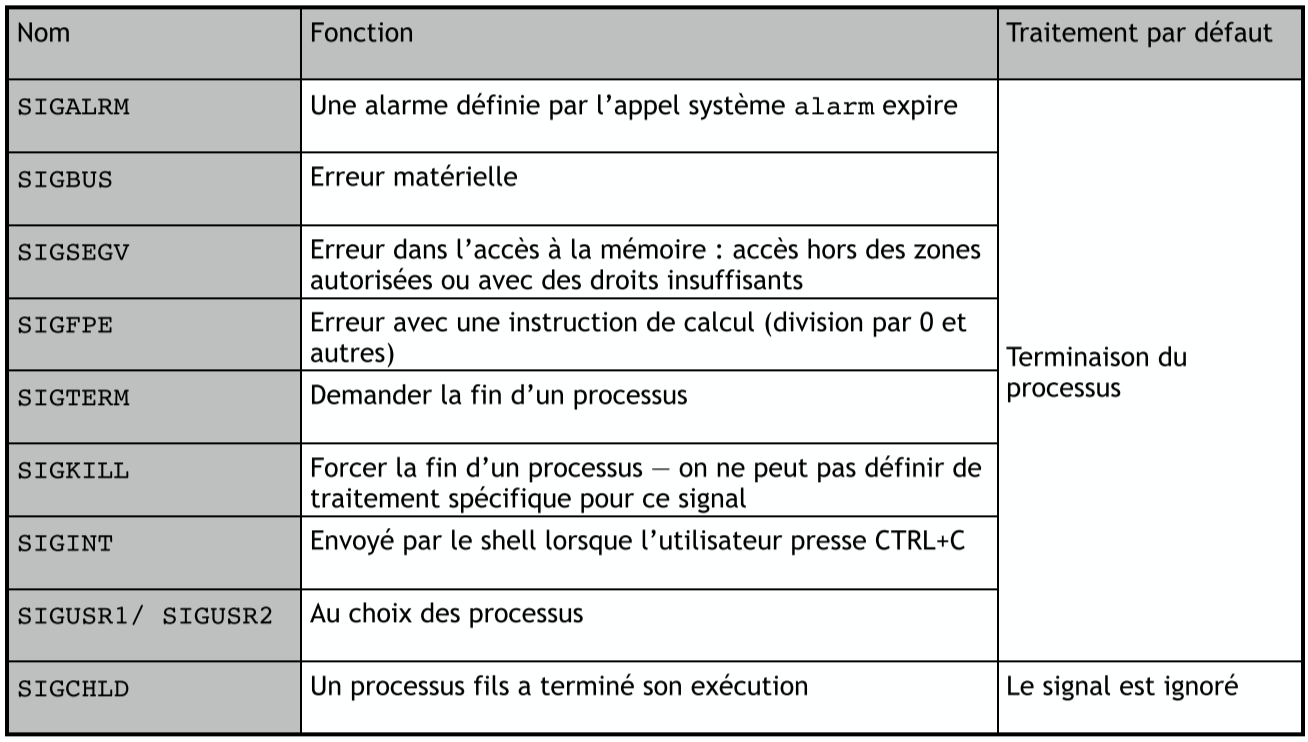
\includegraphics{image-64.png}
\caption{Tableau résumé des signaux communs}
\end{figure}

À noter que \texttt{SIGTERM}, \texttt{SIGKILL} et \texttt{SIGINT} sont
des signaux asynchrones et permettent de terminer un processus
proprement. De plus, \texttt{SIGUSR1} et \texttt{SIGUSR2} est laissé au
choix du processus.

\texttt{SINGINT} est réservé au shell. \texttt{SIGTERM} est mieux que
\texttt{SIGKILL} car on peut programmer un traitement spécifique.
\texttt{SIGKILL} c'est comme un bazooka.

\paragraph{Envoi de signaux}\label{envoi-de-signaux}

\begin{Shaded}
\begin{Highlighting}[]
\PreprocessorTok{\#include }\ImportTok{\textless{}sys/types.h\textgreater{}}\PreprocessorTok{ }
\PreprocessorTok{\#include }\ImportTok{\textless{}signal.h\textgreater{}}

\DataTypeTok{int}\NormalTok{ kill}\OperatorTok{(}\NormalTok{pid\_t pid}\OperatorTok{,} \DataTypeTok{int}\NormalTok{ sig}\OperatorTok{);}
\end{Highlighting}
\end{Shaded}

\texttt{kill} est un nom historique et ne sert pas qu'à tuer un
processus. Comportement spécifique en fonction de \texttt{pid}:

\begin{itemize}
\tightlist
\item
  \texttt{pid\ \textgreater{}\ 0}: envoi au processus spécifié par PID.
\item
  \texttt{pid\ ==\ 0}: envoi à tous les processus du même groupe. (tous
  les processus d'un pipe == même groupe).
\item
  \texttt{pid\ ==\ -1}: envoi à tous les processus pour lesquels le
  processus appelant à le droit d'envoyer un tel signal.
\item
  \texttt{pid\ \textless{}\ -1}: envoi à tous les processus d'un groupe
  spécifique (groupe étant égal à \texttt{\textbar{}pid\textbar{}})
\end{itemize}

\paragraph{Traiter}\label{traiter}

\begin{Shaded}
\begin{Highlighting}[]
\PreprocessorTok{\#include }\ImportTok{\textless{}signal.h\textgreater{}}\PreprocessorTok{ }
\KeywordTok{typedef} \DataTypeTok{void} \OperatorTok{(*}\NormalTok{sighandler\_t}\OperatorTok{)(}\DataTypeTok{int}\OperatorTok{);}

\NormalTok{sighandler\_t signal}\OperatorTok{(}\DataTypeTok{int}\NormalTok{ signum}\OperatorTok{,}\NormalTok{ sighandler\_t handler}\OperatorTok{);}
\CommentTok{/*}
\CommentTok{* signum:  numéro du signal à traiter}
\CommentTok{* handler: c\textquotesingle{}est une fonction de gestion qui prend un int}
\CommentTok{*/}
\end{Highlighting}
\end{Shaded}

exemple:

\begin{Shaded}
\begin{Highlighting}[]
\DataTypeTok{volatile} \DataTypeTok{sig\_atomic\_t}\NormalTok{ n\_sigusr1}\OperatorTok{=}\DecValTok{0}\OperatorTok{;} 
\DataTypeTok{volatile} \DataTypeTok{sig\_atomic\_t}\NormalTok{ n\_sigusr2}\OperatorTok{=}\DecValTok{0}\OperatorTok{;}

\DataTypeTok{static} \DataTypeTok{void}\NormalTok{ sig\_handler}\OperatorTok{(}\DataTypeTok{int}\OperatorTok{);} 

\DataTypeTok{int}\NormalTok{ main }\OperatorTok{(}\DataTypeTok{int}\NormalTok{ argc}\OperatorTok{,} \DataTypeTok{char} \OperatorTok{*}\NormalTok{argv}\OperatorTok{[])} \OperatorTok{\{}
  \ControlFlowTok{if}\OperatorTok{(}\NormalTok{signal}\OperatorTok{(}\NormalTok{SIGUSR1}\OperatorTok{,}\NormalTok{sig\_handler}\OperatorTok{)==}\NormalTok{SIG\_ERR}\OperatorTok{)} \OperatorTok{\{} \OperatorTok{(...)} \OperatorTok{\}} 
  \ControlFlowTok{if}\OperatorTok{(}\NormalTok{signal}\OperatorTok{(}\NormalTok{SIGUSR2}\OperatorTok{,}\NormalTok{sig\_handler}\OperatorTok{)==}\NormalTok{SIG\_ERR}\OperatorTok{)} \OperatorTok{\{} \OperatorTok{(...)} \OperatorTok{\}}

  \ControlFlowTok{while}\OperatorTok{(} \OperatorTok{(}\NormalTok{n\_sigusr1}\OperatorTok{+}\NormalTok{n\_sigusr2}\OperatorTok{)} \OperatorTok{\textless{}}\DecValTok{5}\OperatorTok{)} \OperatorTok{\{} 
    \CommentTok{// vide}
  \OperatorTok{\}}

\NormalTok{  printf}\OperatorTok{(}\StringTok{"Fin du processus}\SpecialCharTok{\textbackslash{}n}\StringTok{"}\OperatorTok{);} 
\NormalTok{  printf}\OperatorTok{(}\StringTok{"Reçu }\SpecialCharTok{\%d}\StringTok{ SIGUSR1 et }\SpecialCharTok{\%d}\StringTok{ SIGUSR2}\SpecialCharTok{\textbackslash{}n}\StringTok{"}\OperatorTok{,}\NormalTok{n\_sigusr1}\OperatorTok{,}\NormalTok{n\_sigusr2}\OperatorTok{);} 
  \ControlFlowTok{return}\OperatorTok{(}\NormalTok{EXIT\_SUCCESS}\OperatorTok{);}
\OperatorTok{\}} 

\DataTypeTok{static} \DataTypeTok{void}\NormalTok{ sig\_handler}\OperatorTok{(}\DataTypeTok{int}\NormalTok{ signum}\OperatorTok{)} \OperatorTok{\{}
  \ControlFlowTok{if}\OperatorTok{(}\NormalTok{signum}\OperatorTok{==}\NormalTok{SIGUSR1}\OperatorTok{)} \OperatorTok{\{} 
\NormalTok{    n\_sigusr1}\OperatorTok{++;}
  \OperatorTok{\}} \ControlFlowTok{else} \OperatorTok{\{}
    \ControlFlowTok{if}\OperatorTok{(}\NormalTok{signum}\OperatorTok{==}\NormalTok{SIGUSR2}\OperatorTok{)} \OperatorTok{\{} 
\NormalTok{      n\_sigusr2}\OperatorTok{++;}
    \OperatorTok{\}} \ControlFlowTok{else} \OperatorTok{\{} 
      \DataTypeTok{char} \OperatorTok{*}\NormalTok{msg}\OperatorTok{=}\StringTok{"Reçu signal inattendu}\SpecialCharTok{\textbackslash{}n}\StringTok{"}\OperatorTok{;} 
\NormalTok{      write}\OperatorTok{(}\NormalTok{STDERR\_FILENO}\OperatorTok{,}\NormalTok{msg}\OperatorTok{,}\NormalTok{strlen}\OperatorTok{(}\NormalTok{msg}\OperatorTok{));} 
\NormalTok{      \_exit}\OperatorTok{(}\NormalTok{EXIT\_FAILURE}\OperatorTok{);}
    \OperatorTok{\}}
  \OperatorTok{\}}
\OperatorTok{\}}
\end{Highlighting}
\end{Shaded}

Cette procédure de traitement peut intervenir à tout moment. Cette
routine d'exécution se fait \textbf{d'une traite}. On ne peut
qu'utiliser des variables globales et \texttt{volatile} empêche la
sauvegarde dans un registre. Pour éviter tout chargement avant le
traitement du signal on utilise \texttt{sig\_atomic\_t}. On ne peut que
faire des appels systèmes et de la librairie ré-entrant.

\subsubsection{Mise en Oeuvre des Signaux dans le
Kernel}\label{mise-en-oeuvre-des-signaux-dans-le-kernel}

2 options:

\begin{enumerate}
\def\labelenumi{\arabic{enumi}.}
\tightlist
\item
  Conserver un fichier par processus pour stocker les signaux qui lui
  sont destinés: pas de perte de signal mais le fichier doit être
  \textbf{vérifié à chaque restauration de contexte}.
\item
  Mot binaire (sous Linux) pour chaque processus avec un bit par signal
  possible. Moins de mémoire utilisée mais pas de garantie sur la
  délivrance des signaux reçus en plusieurs exemplaires.
\end{enumerate}
